
\chapter{CGAL 3D Viewer}

\section{Introduction}
\ccc{Viewer\_3} is a CGAL class that implements a three dimensional viewer for 
geometric objects. It is based on OpenGL for the graphic part and FLTK 
(Fast Light Tools Kit)
for the window, the widgets and the events handling. \\
As it uses OpenGL graphic capabilities, the viewer can display
3-dimensional objects with full graphic quality (including lights,
material properties, textures, special effects as blending
or fog...). Obviously, the cost in time computation is proportional
to the quality of the rendering.\\
The FLTK library provides all the necessary tools to add
interacivity to the interface : buttons, menu bars, sliders,
browsers, windows and subwindows, mouse events handling...\\
The class \ccc{Viewer\_3} is build as a multithreading application. The avantage is 
that the main function can be interrupted easily with a stop signal,
giving control to the viewer thread. A simple click on the viewer
``Exit thread'' button suspends the viewer thread and wakes up the main
one. As some platform doesn't support multithreading application, a
flag \ccc{USE\_THREAD} has to be set in the makefile to allow
multithreading functionnalities.\\
Graphical geometric objects inherit from a virtual class 
\ccc{Drawable\_object}. All of them have the same interface. They are stored by the
viewer in a two level scene graph that can be accessed interactively
with the viewer window or by functions in the main program. \\
In order to use the \ccc{Viewer\_3}, you will need to install the FLTK
library (http://www.fltk.org/about.html) and the OpenGL (or Mesa)
library (http://www.opengl.org/, http://mesa3d.sourceforge.net/).


\section{Global view}
\begin{ccTexOnly}
\begin{center}
\includegraphics[width=10cm]{viewer.eps}
\end{center}
\end{ccTexOnly}
\begin{ccHtmlOnly}
<CENTER>
<img border=0 src=viewer.gif align=center alt="The wiever"> 
</CENTER>
\end{ccHtmlOnly}



The package contains two major classes : \ccc{Viewer\_3} and 
\ccc{GL\_win}. Two more classes implement the scene graph : \ccc{Scene\_graph} and \ccc{Scene\_group}. Several classes are provided to
define drawable objects which inherit from a single virtual class :
\ccc{Drawable\_object}. 

\subsection{The viewer class and window}

The \ccc{Viewer\_3} constructor takes one argument, the scale of the scene to
be visualized. The user has to give a inetger value that match the
coordinates of its datas. 
\\
By default, the size of the window is a square of 600
pixels but it can be reshaped as needed. \\
The main data member (except all the widgets) is a \ccc{GL_win}
visualization window to
display the drawable objects into. Some functions are provided to interact
with the OpenGl window (\ccc{display, add\_drawable,
remove\_drawable}) or get its reference.

\subsection{The OpenGL window : \protect \ccc{GL_win}}

The class \ccc{GL\_win} implements an FLTK window to visualize OpenGL
drawing. In fact, it is more than that, because it contains
the scene graph, the projection and transformations parameters, the
information on how mouse events are interpreted inside the window,
light definition and modification...\\
The \ccc{GL\_win} contains all the information it needed to draw the
scene graph and interact with it.

\subsection{The scene graph}

This is the container for drawable objects. The scene graph is a
member of the \ccc{GL\_win} and contains
scene groups (class \ccc{Scene\_group}) that store pointers to
drawable objects (because \ccc{Drawable\_object} is a virtual class,
all the objects that inherit from it must be use by reference for
correct function calls). Each scene group has its proper matrices for
transformation and stores information about the visibility of each
object. The scene graph panel modes allow to ``hide'' non selected
objects groups, by assigning their visibility status to false.

\subsection{The drawable object}

Each drawable object inherits from the virtual class 
\ccc{Drawable\_object}. A drawable object knows few things : its coordinates 
(eventually a pointer to a CGAL object for complex structures), its
center (a point used by the scene graph to compute the center of
rotation for the whole scene), how to draw itself and eventually how to add a
new point if the drawable object has a \ccc{add_point()} method
implemented (the corresponding \cgal\ object sould handle point
insertion).

\section{The viewer interface}

Within the viewer window several modes and actions are provided. In
all cases (except in user mode or if the ``Group tranforms'' mode is
on) the left mouse button controls global translation and the middle
one global rotation. Two sliders provide control on the viewing
perspective and it is possible to switch from orthogonal to 
perspective projection. 

\subsection{General parameters}

The viewer provides a panel to control the scene lightning (``Set
light''). Another panel is provided to set parameters as the default
parameters for drawable objects. The viewer stores two colors, a
precision, a style and a size parameters that can be assign to
drawable objects as default parameters. They is also a panel to control cliping planes (``Cliping''). \\
A button (``Exit Thread'') stops the viewer thread and gives back the
control to the main thread. The ``Reset'' button sets all the
transformation matrices (translation, rotation) to identity.

\subsection{Viewer global modes}

Four global modes are implemented. 
\begin{description}
\item{$\triangleright$} {\bf View : } This is the standard mode for
visualization. Objects are displayed in the \ccc{GL_win} window and
the mouse handles translation (left button) and rotation (middle button).
\item{$\triangleright$} {\bf Insert point : } This mode allow the user 
to add a point (to the scene graph or to a specific - selected -
object). A transluent plan is drawn and user can move the
plan (with the roller under the window), the scene and an additional point to
place it where he wanted to. Using the menu ``Insert'', the point is
inserted in the first selected group (``In group''), in a new group
(``In new group'') or into a selected drawable object that implement a point
insertion (``In object''). If no such implementation is provided,
nothing is done. The new point can be moved in its support plane by
using right mouse button.
\item{$\triangleright$} {\bf Slice : } Clips the scene with two
cliping planes, displaying only a slice of the scene. The slice
(width, coordinates, direction) is controlled by the ``Cliping''
panel.
\item{$\triangleright$} {\bf User mode : } The user mode switches
mouse events from standard mode to user defined mouse events (user
have to implement how mouse event are handled).  
\end{description}


\subsection{The scene graph browser and modes}

A browser (on the left), a ``Graph'' and a ``View mode'' menu 
allow the user to interact with the scene graph. All the groups 
and the drawables they contain are displayed in the
browser. Selections can be made via clicking on groups in the browser
and actions can occur on them via the ``Graph'' menu : remove
selected drawable, reset local transformation for the first selected group, 
add new group).\\
The ``View mode'' allows to set how the scene graph has to be viewed : 
all drawables are displayed, only selected groups are displayed,
transformations occur locally on selected groups, selected groups are 
highlighted. \\
Objects can move from group to group by using the up and down arrows
on the left of the browser.

\subsection{The user panel}

Users can define their own buttons and actions in a special panel
activated by the the ``User Panel'' button. By default, there is nothing 
but a ``Close'' button in this panel.

\section{The drawable objects}

The class \ccc{Drawable\_object} provides the interface for all user
defined drawable objects. Actually, a file \ccc{draw_CGAL_Objects.h}
implements this interface and provides drawable objects for the CGAL
kernel objects in two and three dimensions.\\
The constructor of a drawable object takes several arguments as :
a reference to a \cgal\ object, two colors, a style, parameter and a
precision parameter.

Actually, color can be defined using the class \ccc{Color} (Color.h) with
RGBA values. we provide some predefined colors : RED, GREEN, BLUE,
ORANGE, VIOLET, PURPLE, DEEPBLUE, GRAY, BLACK, WHITE.\\
How the style parameter is handled depends of the specific drawable
object implementation. FILL means generally nice, filled, solid
object. WIRE is often what it usually means and RAW is the costeless
(in computation time) way to define an object (but the worst in terms
of rendering).\\
The precision is important in FILL style (sometimes in WIRE style
too) because it sets how many facets will model the object. The size
parameter 
sets the line width for WIRE and RAW style and the width of a drawable
point. \\
All drawable objects must implement their constructors, their
\ccc{set\_center()} and \ccc{draw()} functions. If it is suitable for
the object, \ccc{add\_point()} could be provided.\\
The best way to write your own drawable objects is to have a look to
the ones that are already implemented. It could be useful to learn a 
little bit of OpenGL if a special rendering is wanted.

\subsection{Adding object into the scene graph}

To add drawable objects to the scene graph, the \ccc{Viewer\_3} class 
provides a function \ccc{add\_drawable\_object(Drawable\_object *,
int)}. We recall that the scene graph contains only pointers to
drawable objects for polymorphism to be effective. The second
argument (an int) specifies the group where the user want to put the
object. \\
For usability reason, we provide stream-like function to send 
CGAL object directly to the scene graph. In this case, the drawable is built
using the viewer default values for color, size, style and
precision. All objects are added in the first object
group. Stream-like functions are provided too for modifying these
viewer values using manipulators.

\subsection{Defining your own drawable object}

To define and implement your own drawable object you have to proceed
as follow : \\
Add a new class that inherits from \ccc{Drawable\_object}, implement
what is needed by this class : specific data members, constructors,
\ccc{set\_center()} and \ccc{draw()} functions...\\
Write a \ccc{convert\_type} function that converts your geometric object into
a drawable object using the viewer default parameters (see Stream support). That's all.

\section{User defined event and action}

Users can defined their owns mouse events when the viewer is set in
``User mode''. To do that, they have to implement their own \ccc{mouse\_push},
\ccc{mouse\_release} and \ccc{mouse\_grab} functions. These functions must have
the following signatures :

\ccc{void my\_mouse\_push(int x, int y, int but, GL\_win * w);}\\
\ccc{void my\_mouse\_release(int x, int y, int but, GL\_win * w);}\\
\ccc{void my\_mouse\_grab(int x1,int y1,int x2,int y2,int dx ,int dy,int but,GL\_win * w);}


The ``push'' and release functions catch the x/y-coordinates (in
screen coordinates) where the mouse is actived. The \ccc{but}
parameter gives witch mouse button has been activated (1,2 or 3). The forth
parameter is a pointer on the \ccc{GL_win}.\\
The ``grab'' function gives the coordinates of the initial click
(x1,y1), the coordinates of the current position (x2,y2) and
difference between two positions (dx,dy) for one event loop. The last
two parameters are the same as previouly.\\
To register these events, the \ccc{Viewer\_3} class provides three
functions : 


\ccc{typedef void (*Mouse\_click)(int , int , int , GL\_win *);}  \\
\ccc{typedef void (*Mouse\_grab)(int ,int,int,int,int,int,int,GL\_win *);} \\
\ccc{void set\_mouse\_push\_handler(GL\_win::Mouse\_click);}\\
\ccc{void set\_mouse\_grab\_handler(GL\_win::Mouse\_grab);}\\
\ccc{void set\_mouse\_release\_handler(GL\_win::Mouse\_click);}\\


Users can build their owns widgets panel and add callback for them
too. They have to define a new function with the following signature :


\ccc{void my\_panel(GL\_win* win, Viewer\_3* view)}

The body will define a new {\tt Fl\_Window} and new widgets with their 
callback functions.\\
To register the new panel to the viewer use the function :


\ccc{typedef void (*User\_ctr\_win)(GL\_win *,Viewer\_3 *);} \\
\ccc{void set\_custom\_panel(User\_ctr\_win\ fct);} 

Examples of user defined events and user defined button panel are
provided in the examples section.

\begin{ccClass}{Viewer_3}
\section{The Viever Class \protect \ccClassTemplateName}

This is the main class that implements the viewer by itself. It
contains several widgets (and associated callback functions) to
interact whith it and a \ccc{GL\_win} to display OpenGL graphic
commands. The \ccc{GL\_win} has a fixed size but its scale (the
dimension of the effective viewing volume) can be defined as a
parameter in the \ccc{Viewer\_3} constructor. The origine of the
system of coordinates is approximativelly (depend on the perspective
choosen) put in the middle of the viewing cube.

\ccInclude{CGAL/Viewer_3.h}

\ccTypes
\ccThree{typedef void (*User_ctr_win User_ctr_win and so on }{}{A
function pointer and so on and so on and so on}
\ccThreeToTwo
 
\ccTypedef{typedef void (*User_ctr_win)(GL_win *,Viewer_3 *) User_ctr_win;}{A
function pointer used as type for the member function
\ccc{set\_custom\_panel(User\_ctr\_win)}.}




\subsection{Functionalities}

\ccCreation
\ccCreationVariable{w}
\ccThree{Viewer_3();}{t = tr bidulebidulebidulebidule}{}
\ccThreeToTwo
\ccConstructor{Viewer_3();}{Defines and displays a new viewer with a
viasualization window scaled on a 500~$\times$~500~$\times$~500 units cube. }

\ccConstructor{Viewer_3(int scale);}{Defines and displays a new viewer scaled on a scale~$\times$~scale~$\times$~scale units cube.}

\ccConstructor{Viewer_3(int x, int y, int z);}{Defines and displays a new viewer scaled on a x~$\times$~y~$\times$~z units cube.}

\ccConstructor{Viewer_3(int x_min, int x_max, int y_min, int y_max,
int z_min, int z_max);}{Defines and displays a new viewer scaled on a
(x_max-x_min)~$\times$~(x_max-x_min)~$\times$~(x_max-x_min) units cube 
whose origin is (x_min, y_min, z_min).}

\ccHeading{Adding things}

\ccMethod{void add_group();}{Adds a new empty group at the end of the
scene graph.}

\ccMethod{void add_drawable(Drawable_object* obj, int g=1);}{Adds the
drawable object obj into the group g.}

\ccAccessFunctions

\ccMethod{pthread_t get_window_thread();}{Returns window's thread.}

\ccMethod{Size get_size();}{Returns the default drawable object \ccc{Size}.}

\ccMethod{Style get_style();}{Returns the default drawable object
\ccc{Style}.}

\ccMethod{Precision get_precision();}{Returns the default drawable
object \ccc{Precision}.}

\ccMethod{Color get_color(int i);}{Returns the default viewer first \ccc{Color} if i=1, the second \ccc{Color} elsewhere.}

\ccMethod{GL_win* get_window();}{Returns a pointer on the \ccc{GL\_win} member.}

\ccMethod{int get_group();}{The total number of groups in the scene graph.}

\ccHeading{Setting}

\ccMethod{void reset();}{Sets to identity all transformation
matrices.}

\ccMethod{void reset_groups();}{for all groups, sets all local
transformations matrices to identity.}

\ccMethod{void set_size(Size s);}{Sets the default drawable object \ccc{Size}
to s.}
\ccMethod{void set_style(Style s);}{Sets the default drawable object \ccc{Style}
to s.}

\ccMethod{void set_precision(Precision p);}{Sets the default drawable object
\ccc{Precision} to p.}

\ccMethod{void set_color(Color c, int i);}{Sets the default viewer
first \ccc{Color} to c if i=1, the second elsewhere.}
\ccMethod{void set_custom_panel(User_ctr_win fct);}{Sets the viewer 
user panel to be defined by the function \ccc{fct}.}

\ccMethod{void set_mouse_push_handler(GL_win::Mouse_click hand_fct);}{Sets the
mouse push handler for the user mode menu to be \ccc{hand\_fct} function.}

\ccMethod{void set_mouse_release_handler(GL_win::Mouse_click hand_fct);}{Sets the
mouse release handler for the user mode menu to be\ccc{ hand\_fct} function.}

\ccMethod{void set_mouse_grab_handler(GL_win::Mouse_grab hand_fct);}{Sets the
mouse grab handler for the user mode menu to be \ccc{hand\_fct} function.}

\ccHeading{Insertion, Removal}

\ccMethod{void add_drawable(Drawable_object* obj , int gr=1);}{Adds
drawable \ccc{obj} to the scene graph in group \ccc{gr}.}

\ccMethod{void remove_drawable(int gr, int i);}{Removes in group \ccc{gr}, the
drawable indiced by \ccc{i}.}

\ccMethod{void delete_drawable(int gr, int i);}{Deletes in group\ccc{gr}, the
drawable indiced by \ccc{i}. The drawable is definitely deleted.}

\ccMethod{void delete_selection();}{Deletes selection made in the
viewer graph browser.}

\ccMethod{void delete_group(int g);}{Deletes the group of drawables
indiced by g;}

\ccHeading{Miscellaneous}

\ccMethod{void display();}{Displays the content of the scene graph on
the screen. Necessary to call each time a modification is done on the
scene.}

\ccMethod{void init_window_thread();}{Inits viewer thread. This function
has to be called only if mode multi-threads is choosen.}

\ccMethod{void main_loop();}{Launches the viewer main loop. If
multi-threading is used, then the function \ccc{init\_window\_thread()} will 
automatically calls the \ccc{main\_loop()}. If not, \ccc{main\_loop()} has to be
explicitaly calls at the end of the main program.}

\end{ccClass}

\begin{ccClass}{GL_win}

\section{The GL window class \protect \ccClassTemplateName }


The class \ccc{GL\_win} implements the visualisation window where OpenGL
primitives are displayed. It also contains matrices for tranformation, 
mouse events catched into the \ccc{GL\_win} and associated
callbacks. \ccc{GL\_win} object is the main data member of the class \ccc{Viewer\_3}. For elementary
usage of the viewer, users do not have to interfer with the \ccc{GL\_win}
object and use \ccc{GL\_win} member functions. For developping more advanced 
application (such as defining a custom actions), it could be necessary 
to access some of the \ccc{GL\_win} functions and parameters.

For more information about this class, see the reference manual.
\ccInclude{CGAL/GL_win.h}
\end{ccClass}

\begin{ccClass}{Drawable_object}

\section{The Drawable Object Class and its inherited ones : \protect \ccClassTemplateName}

The class \ccc{Drawable\_object} is a virtual class that implement the
generic representation for a drawable object. All drawable objects
contained in the scene graph derive from this virtual class. The
principal functions it defines are not implemented in the virtual
\ccc{Drawable\_object} class but in its derived classes, as each drawable
has its proper way to draw itself, compute its gravity center and so
on. 

\ccInclude{CGAL/Drawable_object.h}

For streams support and users comfort, some types (\cgal\ types) are
defined :

\ccTypes
\ccThree{typedef unsigned char Precision}{}{The Rendering quality for 
a drawable object.}
\ccThreeToTwo

\ccEnum{enum Style {FILL=1, WIRE, RAW, FOS1, FOS2, FOS3, FOS4, FOS5};}{FILL, WIRE and RAW are standard styles for drawables, and FOS are
special styles for facets objects.}

\ccTypedef{typedef int Size;}{The size of a drawable object.}
\ccGlue
\ccTypedef{typedef unsigned char Precision;}{The Rendering quality for 
a drawable object.}

A drawable object has several data members : two colors, style,
precision and center of mass. It also has an OpenGL display list flag, 
\ccc{lind},  for the object that said if OpenGL display list (to speed up GL
computation) is already computed or not; \ccc{lind} is 0 if the object has
never been drawn (no call to draw function) and 1 when the first call to
draw is made. If the object is change (color, add of point, etc), \ccc{lind}
must be reset to 0 to force the draw function to rebuild the display
list. (see OpenGL programming manual for more information on display
lists).




\ccCreation
\ccCreationVariable{obj}
\ccThree{Drawable_object();}{t = tr bidulebidulebidulebidule}{}
\ccThreeToTwo
\ccConstructor{Drawable_object();}{Empty constructor;}

\subsection{Functionalities}


\ccMethod{virtual void draw();}{Virtual drawing method.}

\ccMethod{void set_center();}{Generic function to compute the gravity
center of the object.}

\ccMethod{double get_center(int i);}{Returns the i-coordinate of the
gravity center (i=0,1,2).}

\ccMethod{void set_style(Style s);}{Sets the objects drawing style to
be s.}
\ccMethod{void set_colors(Color c1, Color c2);}{Sets the color to \ccc{c1} and
the second color to \ccc{c2}.}

\ccMethod{void set_color1(Color c1);}{Sets the first color to \ccc{c1}.}

\ccMethod{void set_color2(Color c1);}{Sets the second color to \ccc{c1}.}

\ccMethod{virtual void add_point(double x, double y, double
z);}{Virtual function to add a point to an object.}

\ccMethod{virtual void to_ps(PS_Stream_3 &ps);}{Virtual function to
send the scene to the postscript stream.}
\end{ccClass}

\subsection{Predifined drawable objects}

The file \ccc{draw\_CGAL\_Object.h} implements several drawable objects 
in two and three dimensions. All these classes are derived (public) from the
virtual interface \ccc{Drawable\_object} and are templated by a geometric
object. All these drawables are using \cgal\ standard acces functions
for accessing coordinates of objects. All coordinates number types
(for the template objects) must support the \cgal\ standard
\ccc{to_double} function. Note that all drawables make a copy of the
\cgal\ object they represent. 

\ccInclude{CGAL/draw\_CGAL\_Object.h}

\subsubsection{Two dimensional objects.}

\ccCreation
\ccCreationVariable{obj}
\ccThree{Drawable_object();}{t = tr bidulebidulebidulebidule}{}
\ccThreeToTwo


\begin{ccClassTemplate}{Drawable_point_2<Point2>}

\ccConstructor{Drawable_point_2(const Point2& p, Color c, Style
		   sty=RAW, Size s = 5 , Precision
		   prec=5);}{Object constructor.The \ccc{Point2} must provide 
 \ccc{x()} and  \ccc{y()} access functions.}


\ccConstructor{Drawable_point_2(const double& x1,const double& y1,
		    Color c, Style sty=RAW, Size s = 5 , Precision
		    prec=5);}{Object constructor. A \ccc{Point_2}
template parameter type on double coordinates must be provided.}
\end{ccClassTemplate}

\begin{ccClassTemplate}{Drawable_segment_2<Segment2>}
\ccConstructor{Drawable_segment_2(const Segment2& sg, Color c, Style
sty= RAW, Size s=2, Precision prec=0);}{The \ccc{Segment2} type must provide
 \ccc{target().x()} and  \ccc{source().y()} access functions.}
\end{ccClassTemplate}


\begin{ccClassTemplate}{Drawable_line_2<Line2>}
\ccConstructor{Drawable_line_2(const Line2& ln, Color c, Style
sty= RAW, Size s=2, Precision prec=15);}{The \ccc{Line2} type must provide
 \ccc{point(int i).x()} acces \ccc{point(int i).y()} access functions.}
\end{ccClassTemplate}

\begin{ccClassTemplate}{Drawable_ray_2<Ray2>}
\ccConstructor{Drawable_ray_2(const Ray2& ry, Color c, Style
sty= RAW, Size s=2, Precision prec=15);}{The \ccc{Ray2} type must provide
 \ccc{point(int i).x/y()} function and source().x/y() function.}
\end{ccClassTemplate}

\begin{ccClassTemplate}{Drawable_triangle_2<Triangle2>}
\ccConstructor{Drawable_triangle_2(const Triangle2& 
tri, Color c1, Color c2=BLACK, Style sty=FILL, Size s=2, Precision prec=0);}{The
\ccc{Triangle2} must provide \ccc{tr[i].x/y()} (i=0,1,2) access functions.}
\end{ccClassTemplate}

\begin{ccClassTemplate}{Drawable_circle_2<Circle2>}
\ccConstructor{Drawable_circle_2(const Circle2& 
crl, Color c, Style sty= RAW, Size s=5, Precision prec=5);}{The
\ccc{Circle2} type must have  \ccc{center().x/y()}  and
\ccc{squared\_radius()} functions.}
\end{ccClassTemplate}


\begin{ccClassTemplate}{Drawable_triangulation_2<Triangulation2>}
\ccConstructor{Drawable_triangulation_2(triangulation_2* tri, Color c1,
Color c2, Style sty=WIRE, Size s=5, Precision prec=15);}{ The
\ccc{Triangulation2} must provide a \cgal\ like interface
(\ccc{Edge_iterator, Vertex_iterator, Vertex_handle, Face_handle} and
functions associated to them).}
\end{ccClassTemplate}

\subsubsection{Three dimensional objects.}

\begin{ccClassTemplate}{Drawable_point_3<Point3>}
\ccConstructor{Drawable_point_3(const Point3 &p, Color c, Style
sty=FILL, Size s=5, Precision prec=15);}{The type \ccc{Point3} must provide
 \ccc{x()},  \ccc{y()},  \ccc{z()} access functions.}
\end{ccClassTemplate}


\begin{ccClassTemplate}{Drawable_point_3<Point3>}
\ccConstructor{Drawable_point_3(const double& x, const double& y,const
double& z, Color c, Style
sty=FILL, Size s=5, Precision prec=15);}{Constructor with three double 
for coordinates. A \ccc{Point_3} template type parameter on double
cordinates must be provided.}
\end{ccClassTemplate}

\begin{ccClassTemplate}{Drawable_points_set_3<InputIterator, Point3>}
\ccConstructor{Drawable_points_set_3(InputIterator first,
InputIterator last, Color c, Style
sty=FILL, Size s=5, Precision prec=15);}{\ccc{first} and \ccc{last}
are iterators on a container containing \ccc{point3} objects.}
\end{ccClassTemplate}

\begin{ccClassTemplate}{Drawable_segment_3<segment3>}
\ccConstructor{Drawable_segment_3(const segment3& sg, Color c, Style
sty=RAW, Size s=5, Precision prec=15);}{The type \ccc{segment3} must
provide \ccc{source()} and \ccc{target()} access functions.}
\end{ccClassTemplate}

\begin{ccClassTemplate}{Drawable_line_3<line3>}
\ccConstructor{Drawable_line_3(const line3& ln, Color c, Style
sty=RAW, Size s=2, Precision prec=15);}{The type \ccc{line3} must
provide \ccc{point(int)} function.}
\end{ccClassTemplate}

\begin{ccClassTemplate}{Drawable_ray_3<line3>}
\ccConstructor{Drawable_ray_3(const ray3& ry, Color c, Style
sty=RAW, Size s=2, Precision prec=15);}{The type \ccc{ray3} must
provide \ccc{point(int)} and source() functions.}
\end{ccClassTemplate}

\begin{ccClassTemplate}{Drawable_triangle_3<triangle3>}
\ccConstructor{Drawable_triangle_3(const triangle3& tri, Color c, Style
sty=WIRE, Size s=2, Precision prec=0);}{The type\ccc{triangle3} must
provide \ccc{tr[i]} for accessing vertices and \ccc{x()},  \ccc{y()},
\ccc{z()} access functions for coordinates of each vertex.}
\end{ccClassTemplate}

\begin{ccClassTemplate}{Drawable_tetrahedron_3<tetrahedron3>}
\ccConstructor{Drawable_tetrahedron_3(const tetrahedron3& tet, Color c, Style
sty=FILL, Size s=2, Precision prec=0);}{The type \ccc{tetrahedron3} must
provide  \ccc{tr[i]} for accessing vertices and  \ccc{x()},
\ccc{y()},  \ccc{z()} access functions for coordinates of each vertex.}
\end{ccClassTemplate}

\begin{ccClassTemplate}{Drawable_triangulation_3<triangulation3>}
\ccConstructor{Drawable_triangulation_3(const triangulation3& tri,
Color c1, Color c2, Style sty=FILL, Size s=2, Precision prec=0);}{The type \ccc{triangulation3} must
provide  \ccc{tr[i]} for accessing vertices and  \ccc{x()},
\ccc{y()},  \ccc{z()} access functions for coordinates of each vertex.}
\end{ccClassTemplate}

\subsubsection{Three dimensional facet objects.}

The file \ccc{facet\_object.h} implements a special kind of drawable object : 
a generic implementation for 3-dimensional object that can be
represented with facets (triangulations, polyhedral surfaces,...).
special menu is defined in the viewer window to interact with these
kind of objects, essentially, by offering several predefined way to
display them. 

\ccInclude{CGAL/facet\_object.h}

This file exports several \cgal\ types that are used into the
\ccc{Drawable\_facets\_object\_3} class and have to be used by user to
build the interface between its own geometric objects and a
\ccc{Drawable\_facets\_object\_3}. 

\ccTypes
\ccThree{typedef Gt::Triangleblblblnl}{}{the triangulatiooooooooooooooooooooooo}
\ccThreeToTwo

\ccTypedef{typedef  std::vector<double> vertex ;}{The vertex type.}
\ccGlue
\ccTypedef{typedef  std::vector<vertex> edge ;}{The edge type.}
\ccGlue
\ccTypedef{typedef  std::list<vertex> facet;}{The facet type.}
\ccGlue
\ccTypedef{typedef  std::list<vertex> list_vertices;}{A list of
vertices.}
\ccGlue
\ccTypedef{typedef  std::list<edge>   list_edges;}{A list of edges.}
\ccGlue
\ccTypedef{typedef  std::list<facet>   list_facets;}{Alist of facets.}

The user must provide its own interface between its object and a
\ccc{Drawable\_facets\_object\_3} in the form of three functions :

\ccThree{typedef Gt::Triangle}{}{the triangulatiooooooooooooooooooooooo}
\ccThreeToTwo
\ccFunction{template <class facet_object> list_vertices
get_vertices(const facet_object &fo);} {Returns the list of vertices
of the object \ccc{fo}.}

\ccFunction{template <class facet_object> list_edges get_edges(const
facet_object &fo);} {Returns the list of edges of the object \ccc{fo}.}

\ccFunction{template <class facet_object> list_facets get_facets(const
facet_object &fo);}{Returns the list of facets of the object\ccc{fo}.}

(Warning : this interface may change in futur)

Facet objects of class \ccc{Drawable\_facets\_object\_3} are like regular
drawable objects (inherits from \ccc{Drawable\_object}). They are templated by
the geometric objects and the template class must be the same as the
one given to the three interface function described bellow. The style
can be of five type : \ccc{FOS1}, \ccc{FOS2}, \ccc{FOS3}, \ccc{FOS4} and \ccc{FOS5}. \ccc{FO1} is a raw
wire frame style, \ccc{FO2} adds raw vertices to the previous one, \ccc{FO3} is
wire frame style with only visible edges shown, \ccc{FO4} shows facets and
\ccc{FO5} is a nice wire frame style build with cylinders for edges and
spheres for vertices. 

\begin{ccClassTemplate}{Drawable_facets_object_3<facets_object_3>}
\ccConstructor{Drawable_facets_object_3(const facets_object_3 &obj
,char* name="Facet Object",Color c, Color c2=BLACK, Style sty=FOS1,
Sizes=2, Precision prec=10);}{Builds a new Drawable\_facets\_object\_3.}
\end{ccClassTemplate}

\begin{ccClass}{Scene_graph}
\subsection{The Scene graph Class, \protect \ccClassTemplateName}

The scene graph of the viewer is implemented in the file
\ccc{scene\_graph.h}. It looks like a list of scene groups and acts as a
container for these groups of drawable objects. It contains also the
transformation matrices (rotation, translation) for the scene and the
center of the scene as data members.

\ccInclude{CGAL/scene\_graph.h}

\end{ccClass}
\begin{ccClass}{Scene_group}
\subsection{The scene group, \protect \ccClassTemplateName}

Scene groups are the elementary drawable objects containers. It is
implemented in the file \ccc{scene\_group.h}. An object of class
\ccc{Scene\_group} contains a vector of drawable object, informations about the
visibility of the group and its objects, its center of mass and two
local transformation matrices for rotation and translation. It exports 
its own iterator type to browse through the objects of the group.

\ccInclude{CGAL/scene\_group.h}

\end{ccClass}

\subsection{Stream support}

\cgal\ objects could directly be sended to the viewer via standard
streams. In this case, drawable objects are automatically builded with 
default parameters. Streams are provided for \cgal\ objects (see the
listing bellow), for \ccc{Color}, \ccc{Size} and \ccc{Precision}. For
user defined drawable objects, the implementor must provide a
\ccc{convert_type} for its drawable type that build a drawable object
and send it to the viewer. This function will be automaticaly called
by the stream operator. 

\ccInclude{CGAL/Viewer_stream.h}

\subsubsection{Input streams}

\ccThree{Viewer_3& operator}{operator<<(Viewer_3& W, Style s);}{}
\ccThreeToTwo
\ccFunction{Viewer_3& operator<<(Viewer_3& W, Object o);}
{Sends the object \ccc{o} to the viewer.}

\subsubsection{Convert functions}

The stream operator for a \cgal\ object is defined generically for any 
object type. It calls a function named \ccc{convert_type(Object o,
Viewer_3 &W)} that returns a reference to a drawable object build with
default parameters stored in the viewer. Each \cgal\ object should
implements such \ccc{convert_type} function in order to use the viewer 
stream. 

The interface for such function is as follows :

\begin{cprog} 
template <class R>
Drawable_Object<Object<R> >*
convert_type(Object<R> p, Viewer_3 &W)
{
  Drawable_Object<Object<R> >* d_obj = new
    Drawable_Object<Object<R> >(p,W.get_color(),W.get_style(),W.get_size(),W.get_precision());
  return(d_obj);
}
\end{cprog}

The file \ccc{Viewer_stream.h} provides \ccc{convert_type} functions
for the kernel objects : 

\ccc{Point_3<R>},  \ccc{Segment_3<R>}, \ccc{Triangle_3<R>},
\ccc{Tetrahedron_3<R>}, \ccc{Line_3<R>}, \ccc{Ray_3<R>},
\ccc{Point_2<R>}, \ccc{Segment_2<R>}, \ccc{Line_2<R>}, \ccc{Ray_2<R>},
\ccc{Triangle_2<R>}, \ccc{Circle_2<R>}.

A function that takes a \ccc{std::vector<R>} with three elements and
returns a \ccc{Drawable_point_3} is also provided.

\subsubsection{Manipulators for assigning \protect \ccc{Viewer_3} parameters}

The stream support offer stream facilities to set some Viewer
parameters like default colors, size, precision, etc. It use a manipulator class \ccc{O_manip} that implements
generic stream function :

\ccFunction{Viewer_3& operator<< (Viewer_3& W, const O_manip<Obj>&
m);}{}

In order to use it, a manipulator must be build. The
\ccc{Viewer_stream.h} defines several manipulator constructor for
standards parameters.

\ccFunction{O_manip<Precision> set_precision(Precision i);}{Defines a
manipulator to set the viewer default precision parameter.}
\ccGlue
 \ccFunction{O_manip<Color> set_color1(Color c);}{Defines a
manipulator to set the viewer default first color parameter.}
\ccGlue
 \ccFunction{O_manip<Color> set_color2(Color c);}{Defines a
manipulator to set the viewer default second color parameter.}
\ccGlue
\ccFunction{O_manip<Size> set_size(Size i);}{Defines a
manipulator to set the viewer default size parameter.}
\ccGlue
\ccFunction{O_manip<Style> set_style(Style i);}{Defines a
manipulator to set the viewer default style parameter.}



\subsection{Threads}

In order to run independently from the main program, the viewer, when
it is defined, launches its proper thread. In this way, user can stop
the main process and control the viewer and then get back to the main
program as often as he want. 
The threads package used is the pthread one. It run actually with
Solaris but some problems are known in linux if the library X has not 
been compile with multithreading options. The Viewer\_3 can be use with 
or without multithreading option by simply add a flag when build
object files : simply add -DUSE\_THREAD in your makefile or in the make 
command line. Also, if multithreading is use, the libpthread.so library
have to be added when linking and option -D\_REENTRANT (see example
makefiles).
The pthread package exports several functions working on threads and
we recommand that people that want to build their own mutithreading
structure have a look to the documentation of pthread functions. This
package provides a simple class for the viewer thread in the file
Threads.h. It provides one function called stop() that stops the main
thread giving control to the viewer thread.

\subsection{Examples}

\subsubsection{How to draw some predefined drawable objects.}

\begin{cprog}

#include <CGAL/Cartesian.h>
#include <CGAL/Viewer_stream.h> /* the Viewer_3 header file */
/* CGAL stuff */
typedef CGAL::Cartesian<double> rep_t;
typedef CGAL::Point_3<rep_t> point_t;
typedef CGAL::Segment_3<rep_t> segment;
typedef CGAL::Triangle_3<rep_t> triangle;
typedef CGAL::Tetrahedron_3<rep_t> tetra;
typedef CGAL::Line_3<rep_t> Line;
typedef CGAL::Ray_3<rep_t> Ray;

int main(int argc, char *argv[]) 
{
  CGAL::Viewer_3 W(500); /* build a new Viever_3 */
  W.init_window_thread(); /* Inits the viewer thread */
  stop();                 /* Stops the main thread */
	/* builds some CGAL points */
  point_t p1(100,50,0);
  point_t p2(200,50,0);
  point_t p3(300,50,0);
	/* builds some drawable objects */
  CGAL::Drawable_point_3<point_t> dp1(p1,CGAL::RED,CGAL::FILL,25,5);
  CGAL::Drawable_point_3<point_t> dp2(p2,CGAL::RED,CGAL::FILL,25,15);
  CGAL::Drawable_point_3<point_t> dp3(p3,CGAL::RED,CGAL::FILL,25,30);

  Line ln(point_t(300,300,1),point_t(300,300,-1));
  Ray ry1(point_t(300,300,0), point_t(400,300,0));

  CGAL::Drawable_line_3<Line> dln(ln,CGAL::RED,CGAL::FILL,5,20);
  CGAL::Drawable_ray_3<Ray> dry1(ry1,CGAL::BLUE,CGAL::FILL,5,10);

  triangle tr(point_t(10,10,-200),point_t(300,10,-200),point_t(200,200,-100));
  tetra tet(point_t(100,100,-200),point_t(400,100,-300),
	     point_t(400,300,-100),point_t(250,250, 100));

  CGAL::Drawable_triangle_3<triangle> dtr(tr,CGAL::GRAY,CGAL::FILL);
  CGAL::Drawable_tetrahedron_3<tetra> dtet(tet,CGAL::ORANGE,CGAL::FILL);

  segment s(p10,p11);
  CGAL::Drawable_segment_3<segment> ds1(s,CGAL::VIOLET,CGAL::FILL,5,10);

  std::list<point_t> lp;
  lp.push_back(point_t(10,10,0));
  lp.push_back(point_t(20,20,0));
  lp.push_back(point_t(30,30,0));
  lp.push_back(point_t(40,40,0));
  std::list<point_t>::iterator first=lp.begin(), last=lp.end();
  CGAL::Drawable_points_set_3<std::list<point_t>::iterator,point_t>
             dlp(first,last,CGAL::RED,CGAL::FILL,5,30);
  /* adding drawable in the scene graph */
  W.add_drawable(&dp1);
  W.add_drawable(&dp2);
  W.add_drawable(&dp3);

  W.display(); /* forces the display of the scene graph */
  stop(); /* stops the main thread, user can interact in the viewer window */

  W.add_drawable(&dln,2);
  W.add_drawable(&dry1,2);
  W.display(); 
  stop();
  W.add_drawable(&dtr,3);
  W.add_drawable(&dtet,3);
  W.display(); 
  stop();
  W.add_drawable(&ds1,4);
  W.display(); 
  stop();
  W.add_drawable(&dlp,5);
  W.display();
  pthread_join(W.get_window_thread(), NULL); /* Join the main thread */
	                                     /* and the viewer thread */
}
\end{cprog} 

\subsubsection{Using facet object}

The file get\_data implements the three functions that necessary for
the \ccc{Drawable\_facet\_objects\_3} class to be build.

\begin{cprog} 

/* the file get_data.h */

#include <CGAL/Cartesian.h>
#include <CGAL/Triangulation_3.h>
#include <CGAL/Triangulation_geom_traits_3.h>
#include <CGAL/Delaunay_triangulation_3.h>
#include <CGAL/facet_object.h>

typedef CGAL::Cartesian<double> rep_t;
typedef CGAL::Triangulation_geom_traits_3<rep_t>  traits_3;
typedef CGAL::Triangulation_vertex_base_3<traits_3>     Vb ;
typedef CGAL::Triangulation_cell_base_3<traits_3>       Fb;
typedef CGAL::Triangulation_data_structure_3<Vb,Fb> TDS3 ;
typedef CGAL::Delaunay_triangulation_3<traits_3,TDS3> Delaunay_3;


list_vertices get_vertices(const Delaunay_3 &fo)
{
  typename Delaunay_3::Vertex_iterator vit;
  list_vertices res;
  vertex v(3);
  for (vit=fo.finite_vertices_begin(); vit!=fo.vertices_end();vit++) {
    v[0]=to_double(vit->point().x());
    v[1]=to_double(vit->point().y());
    v[2]=to_double(vit->point().z());
    res.push_back(v);
  }
return res;
}


list_edges get_edges(const Delaunay_3 &fo)
{
  typename Delaunay_3::Edge_iterator it;
  list_edges res;
  edge ed(2);
  vertex vx(3);
  typename Delaunay_3::Cell_handle f;
  int n1, n2;
  typename Delaunay_3::Vertex_handle v1, v2;
  for (it=fo.finite_edges_begin(); it!=fo.edges_end();it++) {
	f = (*it).first;
	n1 = (*it).second;
       	n2 = (*it).third;
	v1 = f->vertex(n1);
	v2 = f->vertex(n2);
    vx[0]=to_double(v1->point().x());
    vx[1]=to_double(v1->point().y());
    vx[2]=to_double(v1->point().z());
    ed[0]=vx;
    vx[0]=to_double(v2->point().x());
    vx[1]=to_double(v2->point().y());
    vx[2]=to_double(v2->point().z());
    ed[1]=vx;
    res.push_back(ed);
  }
return res;
}

list_facets get_facets(const Delaunay_3 &fo)
{
  typename Delaunay_3::Facet_iterator it;
  list_facets res;
  facet fa;
  vertex v(3);
  for (it=fo.finite_facets_begin(); it!=fo.facets_end();it++) {
    fa.clear();
    v[0]=(((*it).first)->vertex(((*it).second +1) &3))->point().x();
    v[1]=(((*it).first)->vertex(((*it).second +1) &3))->point().y();
    v[2]=(((*it).first)->vertex(((*it).second +1) &3))->point().z();
    fa.push_back(v);
    v[0]=(((*it).first)->vertex(((*it).second +2) &3))->point().x();
    v[1]=(((*it).first)->vertex(((*it).second +2) &3))->point().y();
    v[2]=(((*it).first)->vertex(((*it).second +2) &3))->point().z();
    fa.push_back(v);
    v[0]=(((*it).first)->vertex(((*it).second +3) &3))->point().x();
    v[1]=(((*it).first)->vertex(((*it).second +3) &3))->point().y();
    v[2]=(((*it).first)->vertex(((*it).second +3) &3))->point().z();
    fa.push_back(v);
    res.push_back(fa);
  }
return res;
}
\end{cprog} 

And the main program
\begin{cprog} 

#include ``get_data.h''
#include <CGAL/Viewer_stream.h>

typedef CGAL::Point_3<rep_t> point_t;

int main(int argc, char *argv[]) 
{
  CGAL::Viewer_3 W(500);
  W.init_window_thread();
  stop();
  Delaunay_3 tr;
  
  tr.insert(point_t(100,100,100));
  tr.insert(point_t(-100,450,-100));
  tr.insert(point_t(0,0,0));
  tr.insert(point_t(200,-130,170));
  tr.insert(point_t(100,-100,-100));
  tr.insert(point_t(400,100,300));
  tr.insert(point_t(210,140,0));
  tr.insert(point_t(-200,50,310));
  tr.insert(point_t(-100,100,-100));
  tr.insert(point_t(100,-300,0));
  tr.insert(point_t(500,-100,-200));
  tr.insert(point_t(200,140,-200));
  tr.insert(point_t(-140,400,-200));
  tr.insert(point_t(100,-350,0));
  tr.insert(point_t(500,-300,-250));
  tr.insert(point_t(300,-100,250));

  CGAL::Drawable_facets_object_3<Delaunay_3>
                     df(tr,"triangulation3",CGAL::ORANGE,CGAL::BLACK);
  W.add_drawable(&df);
  W.display();
  pthread_join(W.get_window_thread(), NULL);
}

\end{cprog} 

\subsubsection{Usage of streams}
Stream operator \ccc{<<} is used. This a main program without threads.
\begin{cprog} 

#include <CGAL/Cartesian.h>
#include <CGAL/Triangulation_3.h>
#include <CGAL/Triangulation_geom_traits_3.h>
#include <CGAL/Delaunay_triangulation_3.h>
#include <CGAL/Viewer_stream.h>

typedef CGAL::Cartesian<double> rep_t;
typedef CGAL::Point_3<rep_t> point_t;
typedef CGAL::Tetrahedron_3<rep_t> tetra;
typedef CGAL::Triangulation_geom_traits_3<rep_t>  traits_3;
typedef CGAL::Triangulation_vertex_base_3<traits_3>     Vb ;
typedef CGAL::Triangulation_cell_base_3<traits_3>       Fb;
typedef CGAL::Triangulation_data_structure_3<Vb,Fb> TDS3 ;
typedef CGAL::Delaunay_triangulation_3<traits_3,TDS3> Delaunay_3;

int main(int argc, char *argv[]) 
{
  CGAL::Viewer_3 W(500);
  Delaunay_3 tr;  
  tr.insert(point_t(100,100,100));
  tr.insert(point_t(100,100,100));
  tr.insert(point_t(400,100,300));
  tr.insert(point_t(-100,100,-100));
  tr.insert(point_t(100,-300,0));
  tr.insert(point_t(500,-100,-200));
  tr.insert(point_t(-140,400,-200));
  tr.insert(point_t(100,-350,0));
  tr.insert(point_t(500,-300,-250));

  W << CGAL::set_color_1(CGAL::ORANGE) ;
  Delaunay_3::Cell_iterator cit;
  tetra t;
  for (cit = tr.finite_cells_begin(); cit != tr.cells_end(); cit++) {
    t=tr.tetrahedron(cit->handle());
    W << t;
  }
 W.main_loop();
}
\end{cprog} 

\subsubsection{Defining user mouse events and user panel}

This example shows how to use \ccc{set_custom_panel()} and
\ccc{set_mouse_push_handler()} to declare new events and viewer
functionalities. The file \ccc{custom_win.h} implements a function
\ccc{my_panel(GL_win*, Viewer_3*)} that defines a user control
panel. The file \ccc{myhandler} implement a mouse push handler that
redefined how mouse push events are handled in the viewer ``user mode''.

file : myhandler.h
\begin{cprog} 
void myhandler(int x, int y, int but, CGAL::GL_win *W) {
  vector<double> v(3);
  v[0]=x*2; v[1]=y*2; v[2]=0;
  W->add_point_to_object(1,1,v);

}
\end{cprog}

file : custom\_win.h

\begin{cprog} 
#include <CGAL/point_generators_2.h>
#include "triang_2.h"   /*this file defines Drawable_voronoi_2*/


void close_c(Fl_Widget* w, void* v)
{

  Fl_Window* win = (Fl_Window*) v;
  delete win;
}

void tri_cb(Fl_Widget* w, void* v)
{
  CGAL::Viewer_3* win = (CGAL::Viewer_3*) v;
  typedef Triangulation_2::Point Point;
  Triangulation_2* tr= new Triangulation_2();  
  CGAL::Vector_2<rep_t> disp( 425.0, 425.0 );
  CGAL::Random_points_in_square_2<Point,CGAL::Creator_uniform_2<double,Point> >
    g ( 500.0 );
  for (int i=0; i<100; i++)
    tr->insert(*g++ + disp);
  CGAL::Drawable_triangulation_2<Triangulation_2>* dtr = new CGAL::Drawable_triangulation_2<Triangulation_2>(tr,win->get_color(), CGAL::ORANGE,CGAL::RAW, 2);
  win->add_drawable(dtr, win->get_group() + 1);
  win->display();
}


void del_cb(Fl_Widget* w, void* v)
{
  CGAL::Viewer_3* win = (CGAL::Viewer_3*) v;
  typedef Delaunay_2::Point Point;
  Delaunay_2* tr=new Delaunay_2();  
  CGAL::Vector_2<rep_t> disp( 425.0, 425.0 );
  CGAL::Random_points_in_square_2<Point,CGAL::Creator_uniform_2<double,Point> >
    g ( 500.0 );
  for (int i=0; i<100; i++)
    tr->insert(*g++ + disp);
  CGAL::Drawable_triangulation_2<Delaunay_2>* dtr = new CGAL::Drawable_triangulation_2<Delaunay_2>(tr,win->get_color(),  CGAL::ORANGE,CGAL::RAW, 2);
  win->add_drawable(dtr, win->get_group() + 1);
  win->display();
}


void vor_cb(Fl_Widget* w, void* v)
{
  CGAL::Viewer_3* win = (CGAL::Viewer_3*) v;
  typedef Delaunay_2::Point Point;
  Delaunay_2* tr= new Delaunay_2();  
  CGAL::Vector_2<rep_t> disp( 425.0, 425.0 );
  CGAL::Random_points_in_square_2<Point,CGAL::Creator_uniform_2<double,Point> >
    g ( 500.0 );
  for (int i=0; i<100; i++)
    tr->insert(*g++ + disp);
  CGAL:: Drawable_voronoi_2<Delaunay_2>* vo = new CGAL::Drawable_voronoi_2<Delaunay_2>(*tr,win->get_color(), CGAL::RAW, 2);
  win->add_drawable(vo, win->get_group() + 1);
  win->display();
}


void vord_cb(Fl_Widget* w, void* v)
{
  CGAL::Viewer_3* win = (CGAL::Viewer_3*) v;
  typedef Delaunay_2::Point Point;
  Delaunay_2* tr= new Delaunay_2();  
  CGAL::Vector_2<rep_t> disp( 425.0, 425.0 );
  CGAL::Random_points_in_square_2<Point,CGAL::Creator_uniform_2<double,Point> >
    g ( 500.0 );
  for (int i=0; i<100; i++)
    tr->insert(*g++ + disp);
  CGAL::Drawable_voronoi_2<Delaunay_2>* vor = new CGAL::Drawable_voronoi_2<Delaunay_2>(*tr,CGAL::ORANGE, CGAL::RAW, 2);
  win->add_drawable(vor, win->get_group() + 1);
  CGAL::Drawable_triangulation_2<Delaunay_2>* dtr = new
    CGAL::Drawable_triangulation_2<Delaunay_2>(tr,CGAL::BLUE,
					       CGAL::GREEN ,CGAL::RAW, 2);
  win->add_drawable(dtr, win->get_group() );

  win->display();
}




void my_panel(CGAL::GL_win* win, CGAL::Viewer_3* view)
{


 Fl_Window* flwin = new Fl_Window(100,500,"Demo win");

 Fl_Button* tri = new Fl_Button(5,5,80,25,"Triangulation");
 tri->callback(tri_cb,(void *) view);

 Fl_Button* del = new Fl_Button(5,35,80,25,"Delaunay");
 del->callback(del_cb,(void *) view);

 
 Fl_Button* vor = new Fl_Button(5,65,80,25,"Voronoi");
 vor->callback(vor_cb,(void *) view);

 Fl_Button* vord = new Fl_Button(5,95,80,25,"Vor. and Del.");
 vord->callback(vord_cb,(void *) view);


 Fl_Button* close = new Fl_Button(5,470,80,25,"Done");
 close->callback(close_c,(void *) flwin);
    flwin->end();
    flwin->show();

}

\end{cprog}
file : main.C
\begin{cprog}
#include <CGAL/Cartesian.h>
#include <CGAL/Viewer_stream.h>

#include "custom_win.h"
#include "myhandler.h"

int main(int argc, char *argv[]) 
{

  CGAL::Viewer_3 W(500);
  W.init_window_thread();
  W.set_custom_panel(my_panel);
  W.set_mouse_push_handler(myhandler);
  W.display();
  stop();
  pthread_join(W.get_window_thread(), NULL);
}

\end{cprog}

\section{Adresses}

About OpenGL consult the official page : http://www.opengl.org/ \\
For Mesa (a free OpenGL clone), consult :
http://mesa3d.sourceforge.net/ \\
For FLTK (free shareware) : http://www.fltk.org/about.html


